\documentclass[11pt, oneside]{article} 
\usepackage{geometry}
\geometry{letterpaper} 
\usepackage{graphicx}
	
\usepackage{amssymb}
\usepackage{amsmath}
\usepackage{parskip}
\usepackage{color}
\usepackage{hyperref}

\graphicspath{{/Users/telliott_admin/Tex/png/}}
% \begin{center} 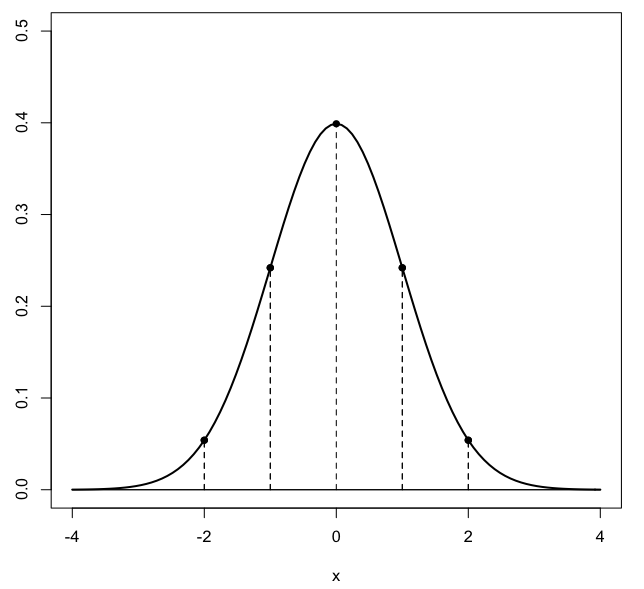
\includegraphics [scale=0.4] {gauss3.png} \end{center}

\title{Integration problems}
\date{}

\begin{document}
\maketitle
\Large

This chapter and the next contain a number of problems which you may find challenging and instructive.  We have reached the end of our discussion of the theory of calculus at this point, though we will see many more applications later.

Definite integrals

\[ \int_{0}^{\pi/2} \cos x \ dx \]
\[ \int_{0}^{\pi/2} \cos \theta \ d\theta \]
\[ \int_{-\pi/2}^{\pi/2} \sin x \ dx \]
\[ \int_0^1 x^2 \ dx \]
\[ \int_0^1 \sqrt{x} \ dx \]

\[ \int_1^{3} \frac{1}{x} \ dx \]
\[ \int_1^2 3x^2 + 2x + 1 \ dx \]

\subsection*{}

\[ \int_{0}^{8} x^{2/3} \ dx \]
\[ \int_{0}^{\pi/4}  \cos 2t \ dt \]
\[ \int_{1}^3 \frac{1}{x^2} \ dx \]

\subsection*{}

\[ \int_0^3 \frac{2t}{1+t^2} \ dt \ ; \ \ \text{hint:  watch the bounds} \]
\[ = \int_{u=1}^{u=10} \frac{1}{u} \ du \]
\[ = \ln u \ \bigg |_{u=1}^{u=10} = \ln 10 - \ln 1 = \ln 10 \]

\subsection*{}

\[ \int_0^1 (3x - 2)^3 \ dx \]
\[ \int_0^1 xe^{-x^2} \ dx \]
\[ \int_{-\pi/4}^{\pi/4} \cos 2x \ dx \]
\[ \int_{-1}^1 xe^x \ dx \]
\[ \int_0^{1/2} \frac{1}{\sqrt{1-x^2}} \ dx \]
\[ \int_0^{e-1} \ln (x + 1) \ dx ; \ \ \text{hint: what is } \frac{d}{dx} x \ln x \ \text{?}\]
\[ \int_{\pi/3}^{\pi/2} \tan \frac{\theta}{2} \ \sec^2 \frac{\theta}{2}\ d \theta \]
\[ \int_{\pi/2}^{x} \cos t \ dt \]
\[ \int_0^{\ln 2} e^{2x} \ dx \]
\[ \int_0^2 (x^3 + k) \ dx = 10 \ ; \ \ \text{find } k \]
\[ \int_0^{\ln 2} e^{2x} \ dx \]
\[ \int_1^e \frac{\ln t}{t} \ dt \]
\[ \int_0^1 x e^{x^2 + 1} \ dx \]

Indefinite integrals

\[ \int \tan x \ dx \]
\[ \int \ln x \ dx \]
\[ \int \sec^2 x \ dx \]
\[ \int \csc^2 \theta \ d \theta \]
\[ \int \tan \theta \sec \theta \ d\theta \]

\subsection*{}

\[ \int (\sqrt{x} + \frac{1}{x^3}) \ dx \]
\[ \int \frac{3x^2 + x - 1}{x^2} \ dx \]
\[ \int \frac{1}{u-3} \ du \]
\[ \int \cos^2(2x) \ \sin 2x \ dx \]
\[ \int \frac{x}{\sqrt{3-4x^2}} \ dx \]
\[ \int \frac{1}{\sqrt{9-x^2}} \ dy \]
\[ \int \frac{x}{(2-x^2)^3} \ dx \]
\[ \int \frac{e^x}{1-2e^x} \ dx \]
\[ \int e^{x + e^x} \ dx \]

\subsection*{}

\[ \int (x^3 - \sin 2x) \ dx \]
\[ \int \frac{e^{3x}}{e^x} \ dx \]
\[ \int \frac{z}{1-4z^2} \ dz \]
\[ \int \frac{5}{1 + x^2} \ dx \]
\[ \int \frac{\cos x}{\sin^2 x} \ dx \]
\[ \int \tan^4 t \ \sec^2 t \ dt \]
\[ \int e^x \cos (e^x) \ dx \]
\[ \int \frac{e^x - e^{-x}}{e^x + e^{-x}} \ dx \]
\[ \int \frac{x+1}{x^2 + 1} \ dx \]
\[ \int \frac{x}{x+a} \ dx \ ; \ \ \text{hint:  } =  \int \frac{x + a - a}{x+a} \ dx \]
\[ \int a^u \ du  \ ; \ \ a = const \]

\subsection*{}

\[ \int e^{4- \ln x} \ dx \]
\[ \int x \ \sqrt{x+2} \ dx \ ; \ \ \text{hint:  } u = x+2 \]
\[ \int \frac{x}{\sqrt{x+3}} \ dx \ ; \ \ \text{hint:  } u = x+3 \]
\[ \int \frac{1+x}{\sqrt x} \ dx \]
\[ \int \frac{1}{x^2 + 2x + 5} \ dx \]
\[ \int \frac{x^2 + 3}{x-1} \ dx \ : \ \ \text{hint:  make top divisible by } x-1 \]
\[ \int \frac{\ln x}{3x} \ dx \]
\[ \int \frac{e^x}{e^x + 1} \ dx \]
\[ \int \frac{1+x}{\sqrt x} \ dx \]
\[ \int \sin \theta \cos \theta \ d \theta \]
for the last, give both versions of the answer and show they are equal

\subsection*{}

\[ \int (\sin x + \cos x)^2 \ dx \]
\[ \int (1 + \tan x)^2 \ dx \]
\[ \int \frac{\cos^2 x}{1 + \sin x} \ dx \]
\[ \int \frac{\sin x}{1 + \sin x} \ dx \]
\[ \int \sin^3 \ dx \]
\[ \int \sec^2 x \ \sqrt{5 + \tan x} \ dx \]
\[ \int \cos x \ e^{1 + \sin x} \ dx \]
\[ \int e^x \cos (e^x) \ dx \]
\[ \int x \sin x \ dx \]
\[ \int e^x \sin x \ dx \]
\[ \int \frac{\sin x + \cos x}{e^{-x} + \sin x} \ dx  \ ; \ \ \text{hint:  multiply by }  e^x/e^x \]
\[ \int \frac{2^{\ln x}}{x} \ dx \]
\[ \int \frac{1}{x \ln x } \ dx \]
\[ \int \frac{\ln \sqrt{x}}{x} \ dx \]

\subsection*{}

For absolute value problems, recall that
 \begin{displaymath}
   |x| = \left\{
     \begin{array}{lr}
       \ \ x & : x \ge 0 \\
       -x & : x < 0
     \end{array}
   \right.
\end{displaymath} 

The method is to find the place where the expression inside the absolute value symbols is equal to zero, then integrate piecewise, substituting as shown above.

\[ \int_0^2 |t-1| \ dt \]

Since $t-1 = 0$ when $t=1$ this is

\[ \int_0^1 -(t-1) \ dt + \int_1^2 (t-1) \ dt \]
\[ = (-\frac{1}{2} t^2 + t) \  \bigg |_0^1 \ + (\frac{1}{2} t^2 - t) \ \bigg |_1^2 \]
\[ = (-\frac{1}{2}  + 1  - 0 + 0) + (2 - 2 - \frac{1}{2} + 1) = 1 \]
Tricky to evaluate.

\subsection*{FTC}

There is a perverse desire to make sure you understand the FTC (part 1).

If $F(x)$ is "nice" and
\[ F(x) = \int_a^x f(t) \ dt \]
then..
\[ F'(x) = \frac{d}{dx} \ F(x) = \frac{d}{dx} \  \int_a^x f(t) \ dt = f(x) \]

Problems:  for each $G(x)$ below, find $G'(x)$

\[ G(x) = \int_1^x 2t \ dt \]
\[ G(x) = \int_0^x (2t^2 + \sqrt{t}) \ dt \]
\[ G(x) = \int_0^x \tan t \ dt \]
\[ G(x) = \int_{x^2}^x \frac{t^2}{1+t^2} \ dt \]

The last problem needs first to be manipulated into a (sum of) integrals between a constant ($0$) on the lower bound and $x$ above, and then the one with $x^2$ must take account of the fact that if $t=-x^2$ then $dt = -2x \ dx$.

\[ G(x) = - \int_0^{-x^2} \frac{t^2}{1+t^2} \ dt +   \int_0^x \frac{t^2}{1+t^2} \ dt \]
\[ G'(x) = - \frac{x^4}{1 + x^4} \ (-2x) + \frac{x^2}{1+x^2} \]

\subsection*{hard one}

Here is a problem involving the actual integral we had above. I didn't know how to solve it completely, but I found the answer on the web and can work backward and see that it's correct.  Call it a challenge.  It looks simple enough:

\[ \int \frac{\sqrt{x}}{1-x} \ dx \]
substitute
\[ u = \sqrt{x}, \ \ u^2 = x, \ \ 2 u \ du = dx \]
we obtain
\[ \int \frac{u}{1-u^2} \ 2 u \ du \]
\[ 2 \int \frac{u^2}{1-u^2} \ du \]

If this were $x$ in the numerator rather than $x^2$, it would be simple.  Still, it looks like it ought to be easy, somehow.  The answer is here:

(http://integrals.wolfram.com/index.jsp)

Let's change to $x$:

\[ \int \frac{x^2}{1-x^2} \ dx \]

The first part of the answer is a useful trick for many problems.  If the numerator is the same as the denominator, within a constant, then:

\[ = - \int \frac{1-x^2 - 1}{1-x^2} \ dx \]
\[ = -\int 1 \ dx - \int \frac{1}{1-x^2} \ dx \]

Now the real trick is that the second part can be re-worked because it is a difference of squares 

\[ (1-x)(1+x) = 1-x^2 \]
\[ \int \frac{1}{1-x^2} \ dx = \frac{1}{2} \int ( \frac{1}{1+x} + \frac{1}{1-x} ) \ dx \]

If we put the two terms on the right over the common denominator $1-x^2$, then for the numerator we have $1-x + 1 + x = 2$.  !!  So the whole integral is

\[ \int \frac{x^2}{1-x^2} \ dx \]
\[ = -x - \frac{1}{2} \ [ \ (\ln (1+x) - \ln(1-x) ) \ ] \ + C \]
\[ = -x - \frac{1}{2} \ \ln \frac{(1+x)}{(1-x)} + C \]

I'll leave it to you to work out the answer to the original problem with $\sqrt{x}$.

\subsection*{another hard one}

\[ \int \frac{\sqrt{x^2 + 1}}{x} \ dx \]

Substitution:  let $x=\tan t$.  So opp = $x$, adj = $1$, hyp = $\sqrt{1 + x^2}$.

\[ x = \tan t \]
\[ dx = \sec^2 t \ dt \]
\[ \sqrt{1 + x^2} = \sec t \]
So the integral is

\[ \int \frac{\sec t}{\tan t} \ \sec^2 t \ dt \]
\[ = \int \frac{\sec t}{\tan t} (1 + \tan^2 t) \ dt \]

The first term is

\[ \int \frac{1}{\sin t} \ dt \]
and the second is

\[ \int \sec t \tan t \ dt \]
\[ = \int \frac{\sin t}{\cos^2 t} \ dt \]

The second part is easy ($1 / \cos t$).  But the first requires more work.  Let 

\[ u = \cos t \]
\[ du = - \sin t \ dt \]

We rewrite the integral as

\[ \int \frac{\sin t}{\sin^2 t} \ dt \]

\[ = - \int \frac{1}{1 - u^2} \ du \]
\[ = - \frac{1}{2} \int \frac{1}{1+u} + \frac{1}{1-u} \ du \]
\[ = - \frac{1}{2} ( \ln (1+u) - \ln (1-u) ) \]

So, in terms of $t$ we have (combining)

\[ \frac{1}{\cos t } - \frac{1}{2} ( \ln (1+\cos t) - \ln (1-\cos t) ) \] 

In order to substitute back to $x$, we recall that

\[ \frac{1}{\sqrt{1 + x^2}} = \cos t \]

and I think we'll just leave it right there.  Well, in the original problem we had a definite integral with limits $\sqrt{15}$ and $\sqrt{3}$, so that $\cos t = 1/4$ at the high end and $\cos t = 1/2$ at the low end which makes it considerably easier to evaluate.

\[ = 4 - \frac{1}{2} (\ln 5/4 - \ln 1/2) - 2 + \frac{1}{2} (\ln 3/2 - \ln 1/2) \]
\[ = 2 - \frac{1}{2}  ( \ln 5/2 +  \ln 3 ) \]



\end{document}  